\section{A social player}
\label{sec:social-player}

First of all, a social player in a card game scenario is basically a player that can interact with other human players in a proper way according to the game situation.
Since its behaviours must be as similar as possible to the interactions of human players, the most expressive robot was chosen to embody this player, \ac{emys}.
Nevertheless, when creating behaviours for an embodied agent, it is important to consider that our perception of a social robot, as a unique entity that interacts, is indeed composed of distinct modules that allow the robot to talk, move, animate, gaze at some point or glance at another.
For this reason, the architecture, presented in Figure\ref{fig:model}, uses \emph{Skene} as its \emph{Behaviour Planner}.
\emph{Skene} has its own language, called utterances, that allow the communication with the robot as a single entity.
These utterances are classified with a category and subcategory and may specify verbal or non-verbal behaviours, as well as both interleaved.
Most of \ac{emys} behaviours in this scenario were conducted by \emph{Skene} due to the provided abstraction while producing complete behaviours (verbal and non-verbal), and also due to the utterances classification that can associate behaviours to game states.
The following subsections will present the main aspects of the utterances list that characterizes \ac{emys} behaviours and the way it will be perceived.
%However, invoking specific instructions without \emph{Skene} can also be directly done

%Additionally, a \emph{Sueca} player has two distinct roles during a game: being partner of his team player and opponent of the other two players.
%With these main concepts in mind, a character of this nature can be developed by specifying its behaviours.
%In other words, considering the connection between the world and the robot is established by \emph{Skene}, this means creating a list of utterances that might contain text to speak, animations, gaze and glance instructions.
%The current section describes the structure of behaviours included in the developed \emph{Sueca} player.


\subsection{\emph{Sueca} behaviours}
The analysis of the card game players on user-centred studies, Chapter~\ref{chapter:user-studies}, revealed key aspects of the interaction during a \emph{Sueca} game.
First of all, there are specific game situations that may cause verbal or non-verbal behaviours.
As a result, these game situations guided the categories and subcategories of the utterances list, presented on the following figure.

\begin{figure}[ht]
	\centering
    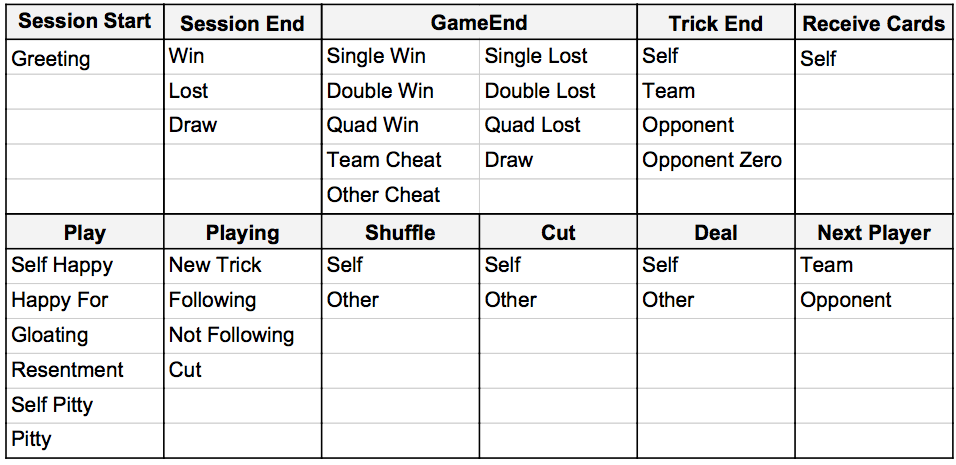
\includegraphics[width=1\textwidth]{./img/6/utterances}
	\caption{Categories and subcategories of the utterances list}
\label{fig:utterances}
\end{figure}

The final list of 205 distinct utterances was inspired by the collected behaviours and replicated to similar ones in order to enrich interactions and to avoid speech redundancies.
The annotated non-verbal behaviours were also applied on \ac{emys} during the same game situations, for instance, looking at a played card and analysing its own hand after that, simulating a re-evaluation of the game.

\subsection{Human-like behaviours}

Besides simply replicating behaviours from human players, there are other things to consider in order to make the robot act as a human, for instance, its speech frequency or its emotional state.
Consequently, this social player applies a probability to decide whether or not to perform an utterance for each game situation.
Additionally, the \emph{FAtiMA} module was used as decision maker of our \emph{Sueca} player, as shown in Figure~\ref{fig:model}, to enrich \ac{emys} presence and allow it to share its emotional state.

\emph{FAtiMA} is a modular architecture for an emotional agent capable of producing 22 different emotions based on its goals and its perceptions of new events for a determined scenario.
Perceptions can be updated by changing the values of 6 appraisal variables (desirability, desirability for other, success probability, failure probability, praiseworthiness and like) and their combination can generate one or more emotions.
However, the current emotional agent of this \emph{Sueca} player is only using 4 appraisal variables, which means it only produces 12 emotions, as presented in Figure~\ref{fig:emotions}.

\begin{figure}[ht]
	\centering
    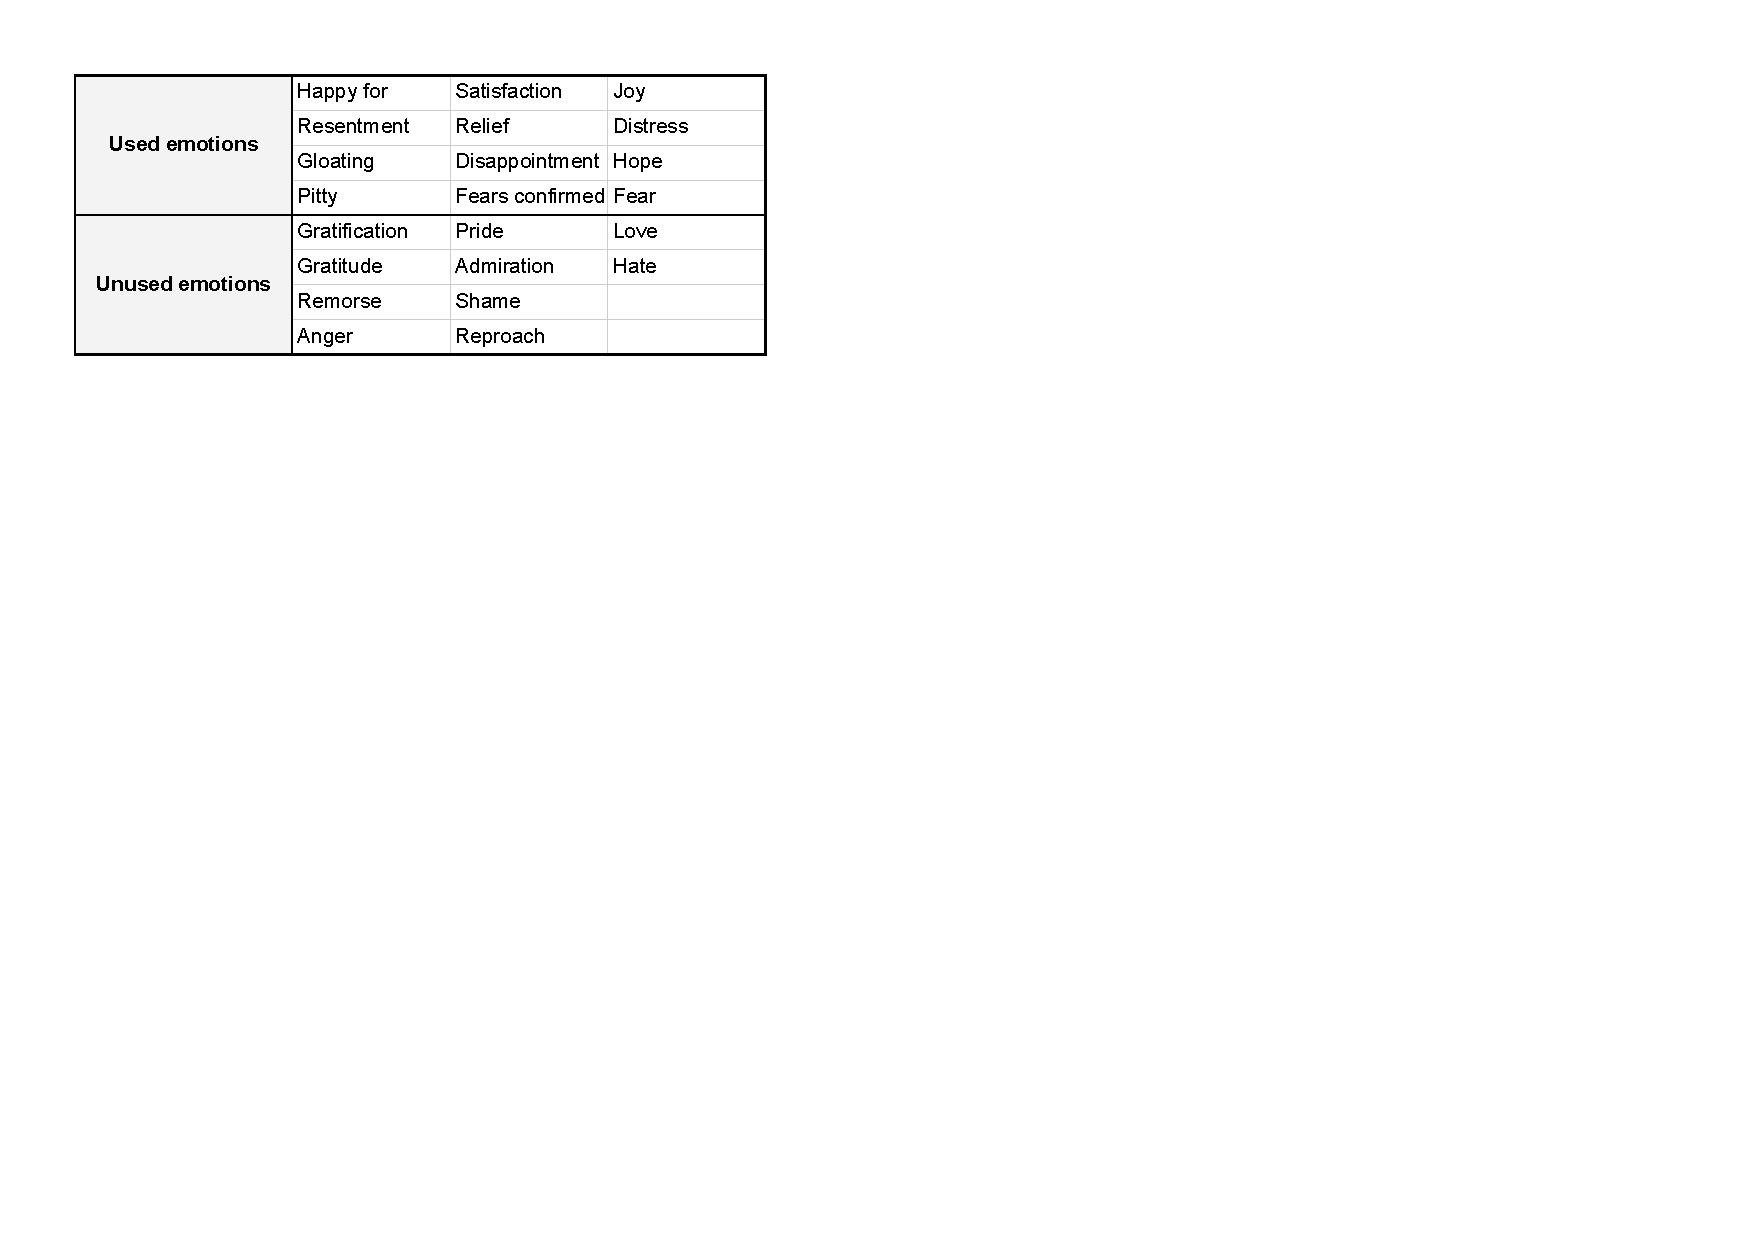
\includegraphics[width=0.75\textwidth]{./img/6/emotions}
	\caption{Distinction of used and non used FAtiMA emotions}
\label{fig:emotions}
\end{figure}

The first approach was to subcategorize utterances with emotional states, however, most of the annotated behaviours by human players evidenced they revealed their emotions in scarce situations during a the game.
A possible reason may lay on the fact that \emph{Sueca} has the element of chance and unknown information should remain hidden.

As a result, emotional states were used on this social player to subcategorize only utterances of the \emph{Play} category.
These utterances are triggered by a play from any player and the idea is to produce an adequate behaviour considering the immediately rewarded benefit.
In other words, each time a player plays a card, the current winner of the trick is computed to analyse how much the agent benefits with that move and also the player itself.
With this strategy, when the agent or its team player make a move, the possible emotions are \emph{Happy For} and \emph{Pitty}, otherwise, when an opponent plays, the possible emotions are \emph{Resentment} and \emph{Gloating}.

Besides the previous usage of the emotional agent, this \emph{Sueca} player is permanently exhibiting its emotional state through its posture.
Since the game success probability is always being updated, together with the mentioned perception of reward, this agent also produces \emph{joy}, \emph{distress}, \emph{hope} and \emph{fear} to set its posture during the game.
%The posture of this embodied agent is an underlying expression over

Finally, another consideration was the opponent and partner component of the \emph{Sueca} game.
From the analysis based on user-centred studies (Chapter~\ref{chapter:user-studies}), annotated verbal behaviours presented some differences between partners and opponent.
For instance, players tend to be more supportive and encouraging to partners and more competitive to opponents.
Theses differences were also included in our \emph{Sueca} player to subcategorize some utterances, as shown in Figure~\ref{fig:utterances}.


\subsection{Enhancing the game interface with behaviours}

Beyond the idea of creating a player that acts humanly in this scenario, other considerations must influence its behaviours.
The final game interface was quite similar to what traditional \emph{Sueca} players are used to, specially due to the usage of physical cards.
However, there are two main concerns to consider when playing over the touch table instead of a traditional \emph{Sueca} game: players must respect their time to play in order for the card to be assumed in the correct order; when a trick has finished, cards must be removed in order to proceed the game.

Consequently, the two utterances' categories differing from analysed human behaviours were \emph{Next Player} and \emph{Trick End}.
The first one is different mainly due to the frequency the agent talks to the next player.
This frequency is higher than the observed by human players in order to enhance this new game experience and encourage players to play on their own times.
The second pointed difference, in \emph{Trick End} utterances, was not taken from user-centred studies.
The pilot experiences evidenced the urge of introducing some cues to remove cards after the trick, and this \emph{Sueca} player warned other players about this.
